\id{МРНТИ 52.35.01}{https://doi.org/10.58805/kazutb.v.1.26-662}

\begin{articleheader}
\sectionwithauthors{А.П. Науанова, Т.О. Хамитова, Н. Парманбек, С. Тянах, Р.З. Касенов, С.Ж. Давренбеков, А.Н. Болатбай, У.Б. Толеуов}{ИССЛЕДОВАНИЕ СВОЙСТВ ГУМИНОВЫХ КИСЛОТ, ПОЛУЧЕННЫХ ИЗ БУРОГО УГЛЯ КУЗНЕЦСКОГО МЕСТОРОЖДЕНИИ}

{\bfseries
\textsuperscript{1}А.П. Науанова\alink{https://orcid.org/0000-0002-5250-1961},
\textsuperscript{1}Т.О. Хамитова\textsuperscript{\envelope } \alink{https://orcid.org/0000-0002-4691-3732},
\textsuperscript{2}Н. Парманбек\textsuperscript{\envelope } \alink{https://orcid.org/00000-0002-9860-1087},
\textsuperscript{3}С. Тянах\textsuperscript{\envelope } \alink{https://orcid.org/0000-0001-5343-4695},
\textsuperscript{3}Р.З. Касенов\alink{https://orcid.org/0000-0002-9832-5115},
\textsuperscript{3}С.Ж. Давренбеков\alink{https://orcid.org/0000-0002-0218-7062},
\textsuperscript{3}А.Н. Болатбай\alink{https://orcid.org/0000-0001-5047-3066},
\textsuperscript{3}У.Б. Толеуов\alink{https://orcid.org/0000-0002-2664-6884}}
\end{articleheader}

\begin{affiliation}
\emph{\textsuperscript{1}Казахский агротехнический исследовательский университет им. Сейфуллина, Астана, Казахстан,}

\emph{\textsuperscript{2}Институт ядерной физики, Алматы, Казахстан,}

\emph{\textsuperscript{3}Карагандинский университет имени Е. А. Букетова, Караганда, Казахстан,}

\raggedright \textsuperscript{\envelope }{\em Корреспондент-автор: \emph{khamitova.t@inbox.ru, \href{mailto:parmanbek.nursanat@gmail.com}{\nolinkurl{parmanbek.nursanat@gmail.com}}, saika\_8989@mail.ru}}
\end{affiliation}

Научная новизна данного исследования заключается в комплексном анализе
физических и химических свойств бурого угля Кузнецкого месторождения с
применением современных методов исследования. Были систематизированы и
представлены данные, касающиеся элементного состава, зольности,
влажности и выхода летучих веществ данного угля. Особое внимание было
уделено изучению влияния функциональных групп на реакционную способность
угля, что ранее не было исследовано в столь детализированной форме для
этого месторождения. Актуальность данного исследования заключается в
глубоком и систематическом анализе свойств гуминовых кислот, полученных
из бурого угля Кузнецкого месторождения, с применением современных
аналитических методов. Впервые в рамках данного исследования были
выявлены и охарактеризованы химические структуры гуминовых кислот, что
позволяет глубже понять их состав и функциональные особенности.
Использование таких методов, как инфракрасная спектроскопия и элементный
анализ, термогравиметрический анализ дало возможность не только
идентифицировать основные функциональные группы бурых углей и гуминовых
кислот, но и определить их термическую стабильность и реакционную
способность. Это позволяет оценить их потенциальное применение в
различных отраслях, таких как агрохимия, экология и медицина. Таким
образом, полученные результаты исследования являются значительным
вкладом в область углехимии и экологии, а также могут послужить основой
для дальнейших исследований и разработок в сфере применения гуминовых
кислот как экологически чистых добавок и сорбентов.

{\bfseries Ключевые слова:} бурый уголь, гуминовые кислоты, кузнецкое
месторождение, функциональные группы, инфракрасная спектроскопия,
элементный анализ, зольность, реакционная способность.

\begin{articleheader}
{\bfseries КУЗНЕЦК ЖӘНЕ КҮМІСҚҰДЫҚ ҚОҢЫР КӨМІРІНЕН СИНТЕЗДЕЛІП АЛЫНАТЫН ГУМИН ҚЫШҚЫЛДАРЫНЫҢ ҚАСИЕТТЕРІН ЗЕРТТЕУ}

{\bfseries
\textsuperscript{1}А.П. Науанова,
\textsuperscript{1}Т.О. Хамитова\textsuperscript{\envelope },
\textsuperscript{2}Н. Парманбек\textsuperscript{\envelope },
\textsuperscript{3}С. Тянах\textsuperscript{\envelope },
\textsuperscript{3}Р.З. Касенов,
\textsuperscript{3}С.Ж. Давренбеков,
\textsuperscript{3}А.Н. Болатбай,
\textsuperscript{3}У.Б. Толеуов}
\end{articleheader}

\begin{affiliation}
\emph{\textsuperscript{1}Сейфуллин атындағы Қазақ агротехникалық зерттеу университеті, Астана, Қазақстан,}

\emph{\textsuperscript{2}Ядролық физика институты, Алматы, Қазақстан,}

\emph{\textsuperscript{3}Е.А.Бөкетов атындағы Қарағанды университеті, Қарағанды, Қазақстан,}

\emph{e-mail: \href{mailto:khamitova.t@inbox.ru}{\nolinkurl{khamitova.t@inbox.ru}}, \href{mailto:parmanbek.nursanat@gmail.com}{\nolinkurl{parmanbek.nursanat@gmail.com}}, saika\_8989@mail.ru}
\end{affiliation}

Бұл зерттеудің ғылыми жаңалығы қазіргі заманғы зерттеу әдістерін қолдана
отырып, Кузнецк кен орнындағы қоңыр көмірдің физикалық-химиялық
қасиеттерін жан-жақты талдауында болып табылады. Бұл көмірдің элементтік
құрамы, күлділігі, ылғалдылығы және ұшпа заттарының шығымы туралы
мәліметтер жүйеленіп, ұсынылып отыр. Бұл кен орны үшін бұрын мұндай
егжей-тегжейлі түрде зерттелмеген көмірдің реактивтілігіне және
функционалдық топтардың әсерін зерттеуге ерекше көңіл бөлінді. Бұл
зерттеудің өзектілігі қазіргі заманғы аналитикалық әдістерді пайдалана
отырып, Кузнецк кен орнының қоңыр көмірінен алынған гумин қышқылдарының
қасиеттерін терең және жүйелі талдауда болып табылады. Бұл зерттеу алғаш
рет гумин қышқылдарының химиялық құрылымын анықтап, сипаттады, бұл
олардың құрамы мен функционалдық сипаттамаларын тереңірек түсінуге
мүмкіндік береді. Инфрақызыл спектроскопия және элементтік талдау және
термогравиметриялық талдау сияқты әдістерді қолдану қоңыр көмір мен
гумин қышқылдарының негізгі функционалдық топтарын анықтауға ғана емес,
сонымен қатар олардың термиялық тұрақтылығы мен реакциялық қабілетін
анықтауға мүмкіндік берді. Бұл олардың агрохимия, экология және медицина
сияқты әртүрлі салаларда әлеуетті қолданылуын бағалауға мүмкіндік
береді. Осылайша, алынған зерттеу нәтижелері көмір химиясы мен
экологиясы саласына қосылған елеулі үлес болып табылады, сонымен қатар
гумин қышқылдарын экологиялық таза қоспалар мен сорбенттер ретінде
пайдалану бойынша одан әрі зерттеулер мен әзірлемелер үшін негіз бола
алады.

{\bfseries Түйін сөздер:} қоңыр көмір, гумин қышқылдары, Кузнецк кен орны,
функционалдық топтар, инфрақызыл спектроскопия, элементтік талдау,
күлділік, реактивтілік.

\begin{articleheader}
{\bfseries STUDY OF THE PROPERTIES OF HUMIC ACIDS FROM BROWN COAL OF THE KUZNETSK DEPOSIT}

{\bfseries
\textsuperscript{1}A.P. Nauanova,
\textsuperscript{1}T.O. Khamitova\textsuperscript{\envelope },
\textsuperscript{2}N. Parmanbek\textsuperscript{\envelope },
\textsuperscript{3}S. Tyanakh\textsuperscript{\envelope },
\textsuperscript{3}R.Z. Kasenov,
\textsuperscript{3}S.Zh. Davrenbekov,
\textsuperscript{3}A.N. Bolatbay,
\textsuperscript{3}U.B. Toleuov}
\end{articleheader}

\begin{affiliation}
\emph{\textsuperscript{1}NCJSC «S.Seifullin Kazakh Agro Technical Research University», Astana, Kazakhstan,}

\emph{\textsuperscript{2}The Institute of Nuclear Physics, Almaty, Kazakhstan,}

\emph{E.A.Buketov Karagandy University, Karaganda, Kazakhstan,}

\emph{e-mail:} \href{mailto:khamitova.t@inbox.ru}{\nolinkurl{khamitova.t@inbox.ru}}, \href{mailto:parmanbek.nursanat@gmail.com}{\nolinkurl{parmanbek.nursanat@gmail.com}}, saika\_8989@mail.ru
\end{affiliation}

The scientific novelty of this research lies in the detailed analysis of
the physical and chemical properties of brown coal from the Kuznetsk
deposit, employing advanced research techniques. Systematic data on the
elemental composition, ash content, moisture content, and volatile
matter yield of this coal have been obtained and presented. Particular
emphasis was placed on examining the influence of functional groups on
coal reactivity---a level of detail previously unexplored for this
deposit. The relevance of this work stems from its in-depth and
structured analysis of the properties of humic acids derived from
Kuznetsk brown coal using modern analytical methods. For the first time,
the chemical structures of humic acids have been identified and
characterized, enabling a more comprehensive understanding of their
composition and functional characteristics. Methods such as infrared
spectroscopy, elemental analysis, and thermogravimetric analysis allowed
for the identification of key functional groups in brown coal and humic
acids, as well as an assessment of their thermal stability and
reactivity. These findings enable an evaluation of their potential
applications in fields such as agrochemistry, environmental science, and
medicine. Consequently, this research makes a substantial contribution
to coal chemistry and environmental studies and provides a foundation
for further research and development on the use of humic acids as
eco-friendly additives and sorbents.

{\bfseries Keywords:} brown coal, humic acids, Kuznetsk deposit, functional
groups, infrared spectroscopy, \\elemental analysis, ash content,
reactivity

\begin{multicols}{2}
{\bfseries Введение.} Гуминовые кислоты, являясь основным компонентом
природного гумуса, играют важную роль в различных биогеохимических
процессах. Они обладают уникальными физико-химическими свойствами, что
делает их перспективными для использования в сельском хозяйстве,
экологии, медицине и промышленности. В последние десятилетия
исследования гуминовых кислот активно развиваются, учитывая их
способность повышать плодородие почвы, стимулировать рост растений,
связывать тяжелые металлы и радионуклиды, а также оказывать
антиоксидантное и иммуностимулирующее воздействие {[}1,2{]}.

Бурый уголь является важным источником гуминовых веществ, и его
переработка позволяет получить гуминовые кислоты в промышленных
масштабах. Одним из перспективных объектов для таких исследований
является бурый уголь Кузнецкого месторождения {[}3{]}. Благодаря своему
химическому составу и доступности, это сырье представляет значительный
интерес для разработки новых экологически чистых технологий получения
гуминовых кислот.

Однако на сегодняшний день изучение свойств гуминовых кислот, полученных
из бурого угля Кузнецкого месторождения, остается недостаточно
исследованным направлением {[}4{]}. Поэтому целью данной работы является
комплексное исследование физико-химических характеристик гуминовых
кислот, извлеченных из этого угля, а также оценка их потенциального
практического применения {[}5,6{]}.

Данная тема актуальна как с точки зрения фундаментальной науки, так и с
точки зрения практических задач, связанных с экологией, сельским
хозяйством и промышленностью. Результаты исследования могут внести
значительный вклад в развитие методов переработки бурого угля и
применения гуминовых веществ в различных сферах {[}7,8{]}.

{\bfseries Материалы и методы.} Объектом исследования в данной работе
является уголь, добываемый на разрезе «Кузнецкий» в Бухар-Жырауском
районе Карагандинской области. Это предприятие входит в число крупнейших
угледобывающих компаний Казахстана и специализируется на добыче бурого
угля марки Б-3. Данный уголь обладает специфическими характеристиками,
такими как низкая зольность (7,4\%), сравнительно высокая влажность
(9,5\%) и значительный выход летучих веществ (47-50\%). Эти параметры
делают его важным ресурсом для энергетики и промышленности региона
{[}9,10{]}.

Применение методов инфракрасной спектроскопии, элементного анализа и
термогравиметрического анализа позволяет не только выявить ключевые
функциональные группы в составе бурых углей и гуминовых кислот, но и
оценить их термическую стабильность и химическую активность. Это
обосновано необходимостью комплексного изучения структуры и свойств
данных веществ для дальнейшего прогнозирования их поведения в различных
процессах.

\emph{Пробоподготовка и анализ исходного сырья.} На начальном этапе
работ нами в качестве исходного сырья для извлечения гуминовых кислот
были взяты образцы бурого угля из Кузнецкого (KUZ) месторождений. Каждый
образец был тщательно измельчен на дробилке марки «Вибротехник ЩД-6» до
фракции 0,5--1 мм для увеличения площади поверхности и облегчения
экстракции (рис.1). Затем угольные образцы были высушены в сушильном
шкафу при температуре 80°C в течение 8 часов для удаления влаги.
\end{multicols}

\begin{figure}[H]
    \centering
    \begin{subfigure}[b]{0.45\textwidth}
        \centering
        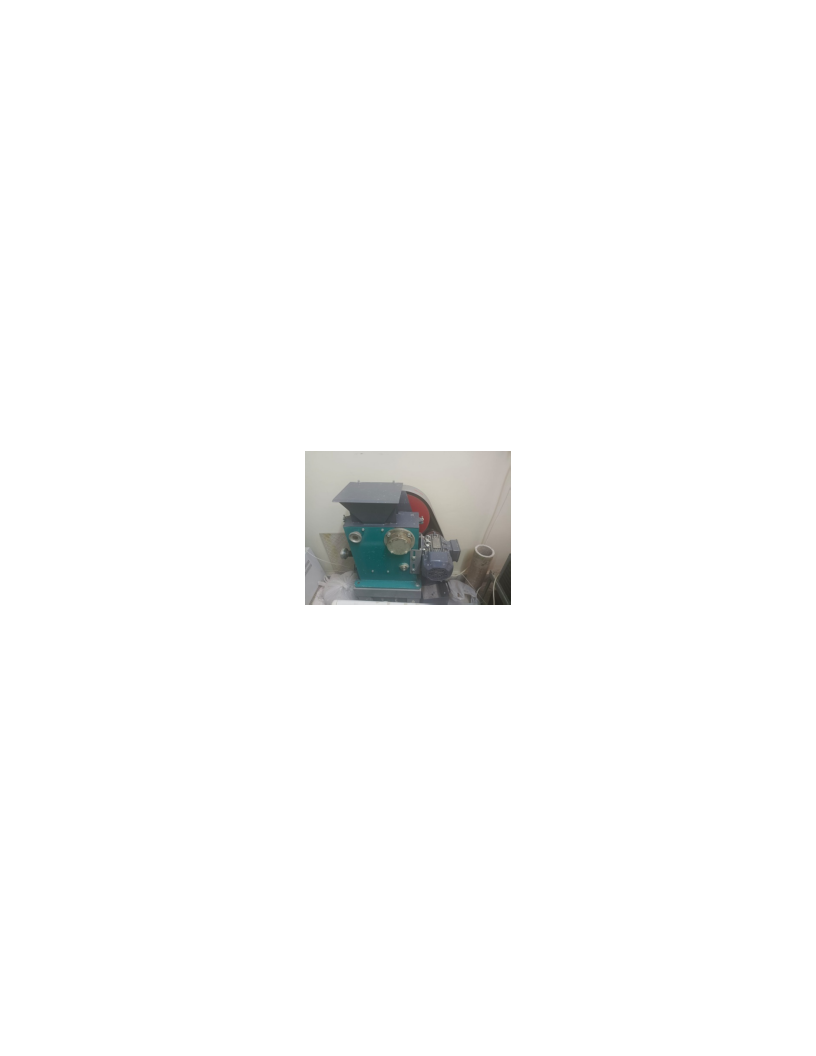
\includegraphics[width=\textwidth]{media/gorn3/image2}
    \end{subfigure}
    ~
    \begin{subfigure}[b]{0.45\textwidth}
        \centering
        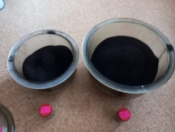
\includegraphics[width=\textwidth]{media/gorn3/image3}
    \end{subfigure}
    \caption*{Рис. 1 - Измельченные и высушенные образцы углей Кузнецкого (KUZ) месторождения}
\end{figure}

\begin{multicols}{2}
\emph{Экстракция гуминовой кислоты из угля водно-щелочным методом.} Для
экстракции гуминовых кислот из бурого угля был использован
водно-щелочной метод с применением гидроксида натрия (NaOH), основанный
на осаждении гуминовых кислот в кислой среде. Гуминовые кислоты были
выделены через реакцию с NaOH, а их разделение в результате осаждения
описывается следующим уравнением:
\end{multicols}

\begin{equation}
\begin{aligned}
\text{Уголь} + \text{NaOH} \text{ ГК-СООNa} + \text{ГМҚ-СООNa} + \text{ФК-СООNa}\\
2\text{ГК-СООNa} + 2\text{ГМК-СООNa} + 2\text{ФК-СООNa} + 3\text{HCl}\\
2\text{ГК-СООNa} + 2\text{ГМК-СООNa} + 2\text{ФК-СООNa} + 3\text{NaCl}
\end{aligned}
\end{equation}

\begin{multicols}{2}
Гуминовые кислоты были экстрагированы путем добавления NaOH к угольным
образцам и последующего осаждения кислым реагентом. В процессе
экстракции 10,0--20,0 г угля с точностью до 0,0001 г помещали в колбу
объемом 250 см³ и добавляли 100 см³ 4\% раствора гидроксида натрия.
Смесь нагревали до температуры 80°C и перемешивали на шейкере в течение
2 часов. Полученную смесь подвергали фильтрации или центрифугированию
для отделения нерастворившихся остатков угля, которые затем промывали
небольшим количеством щелочного раствора. Остатки угля высушивали и
взвешивали для дальнейшего анализа. Измеряли объем экстрагированного
раствора и проводили оценку содержания гуминовых кислот в конечном
продукте (рис.2).
\end{multicols}

\begin{figure}[H]
    \centering
    \begin{subfigure}[b]{0.32\textwidth}
        \centering
        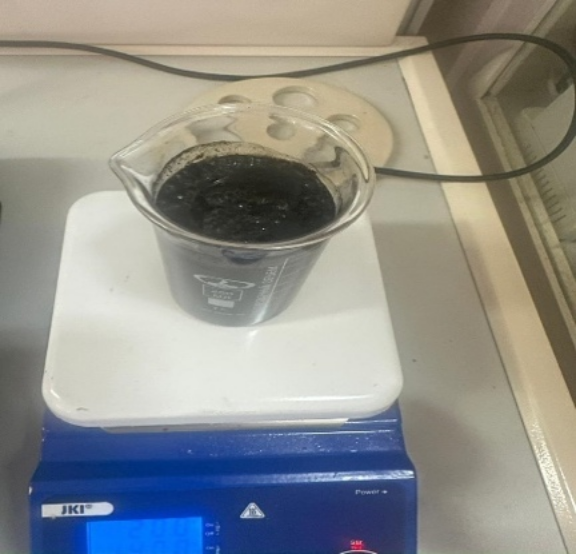
\includegraphics[width=\textwidth, height=\textwidth]{media/gorn3/image4}
    \end{subfigure}
    \begin{subfigure}[b]{0.32\textwidth}
        \centering
        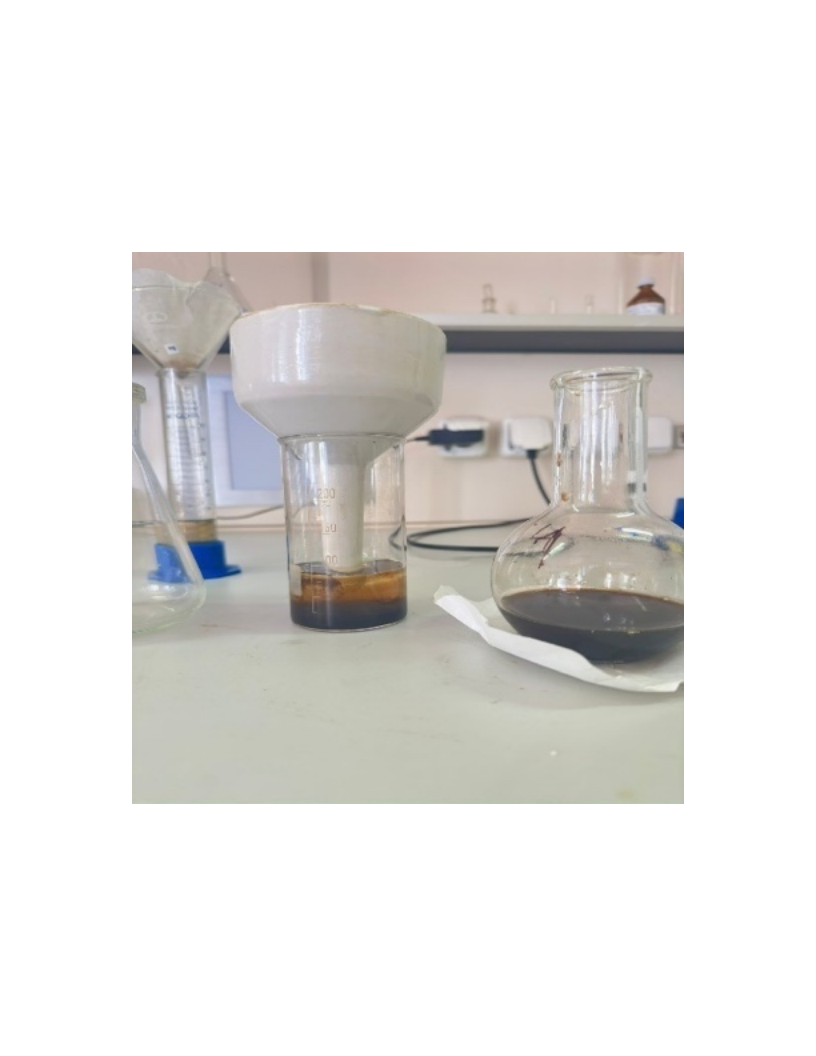
\includegraphics[width=\textwidth, height=\textwidth]{media/gorn3/image5}
    \end{subfigure}
    \begin{subfigure}[b]{0.32\textwidth}
        \centering
        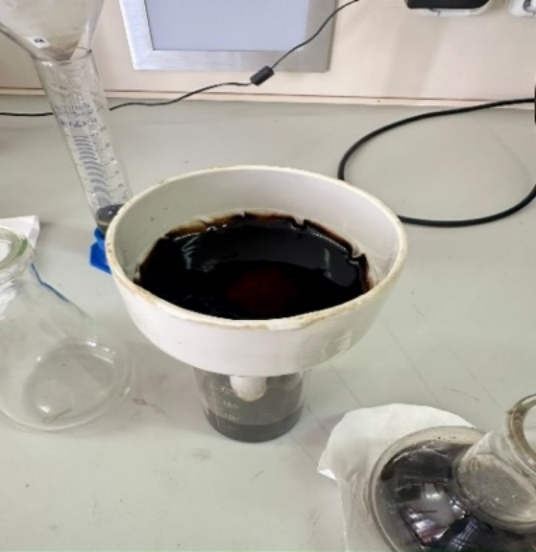
\includegraphics[width=\textwidth, height=\textwidth]{media/gorn3/image6}
    \end{subfigure}
    \begin{subfigure}[b]{0.32\textwidth}
        \centering
        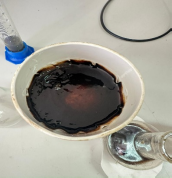
\includegraphics[width=\textwidth, height=\textwidth]{media/gorn3/image7}
    \end{subfigure}
    \begin{subfigure}[b]{0.32\textwidth}
        \centering
        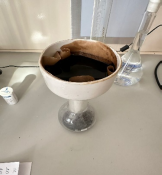
\includegraphics[width=\textwidth, height=\textwidth]{media/gorn3/image8}
    \end{subfigure}
    \begin{subfigure}[b]{0.32\textwidth}
        \centering
        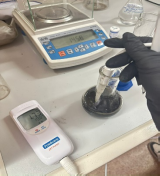
\includegraphics[width=\textwidth, height=\textwidth]{media/gorn3/image9}
    \end{subfigure}
    \caption*{Рис. 2 - Процесс выделения гуминовых кислот из бурых углей}
\end{figure}

\begin{multicols}{2}
Гуминовую кислоту осаждали в 5\%-ном растворе HCl, поддерживая pH смеси
на уровне 2--3. Смесь оставляли для осаждения на 60 минут, после чего
образовавшийся осадок гуминовой кислоты фильтровали через предварительно
взвешенную фильтровальную бумагу (синяя полоска). Осадок тщательно
промывали дистиллированной водой для удаления примесей и остатков
реагентов. После завершения фильтрации, фильтровальную бумагу с осадком
аккуратно извлекали из воронки Бюхнера, складывали в несколько слоев и
предварительно высушивали. Затем фильтр с осадком помещали в заранее
взвешенный стакан и сушили в сушильной печи при температуре 80°C до
достижения постоянной массы. Этот этап обеспечивал полное удаление влаги
из осадка и позволял точно измерить массу выделенной гуминовой кислоты
{[}7,8{]}.

\emph{Элементный состав образцов.} Методика исследования элементного
состава образцов была проведена с использованием органического
элементного анализатора CHNS-O UNICUBE производства компании «Elementar
Analysensysteme GmbH» (Германия). Исследовательская работа была
выполнена в лаборатории Назарбаев Университета (рис.3). Принцип работы
анализатора основан на классическом методе Дюма-Прегля, включающем
сжигание образцов в присутствии окислителя в потоке инертного газа.
Процесс сжигания осуществлялся в динамических условиях, предполагающих
подачу постоянного потока кислорода на протяжении заданного времени, в
результате чего образовывались такие аналитические формы элементов, как
диоксид углерода (CO₂), вода (H₂O), молекулярный азот (N₂) и диоксид
серы (SO₂). Для взвешивания точных навесок применялись аналитические
ультрамикровесы «Mettler Toledo XPR6U Ultra-Microbalance». Образцы
помещались в одноразовые оловянные лодочки толщиной менее 0,01 мм,
которые герметично запечатывались пинцетом для предотвращения утраты
образца {[}7-8{]}.
\end{multicols}

\begin{figure}[H]
    \centering
    \begin{subfigure}[b]{0.45\textwidth}
        \centering
        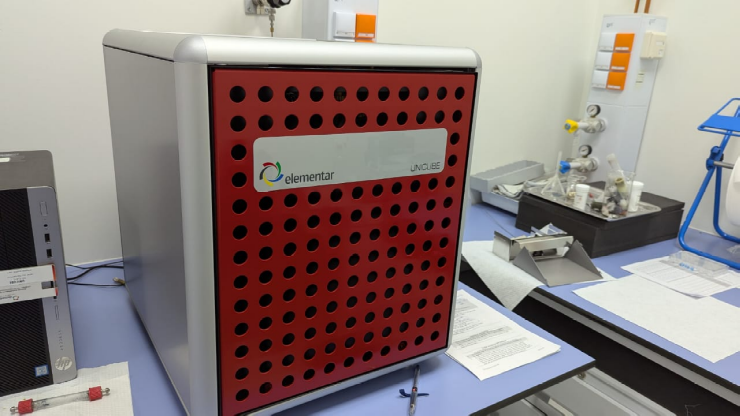
\includegraphics[width=\textwidth]{media/gorn3/image10}
    \end{subfigure}
    \begin{subfigure}[b]{0.45\textwidth}
        \centering
        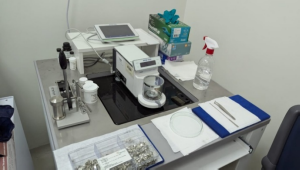
\includegraphics[width=\textwidth]{media/gorn3/image11}
    \end{subfigure}
    \caption*{Рис. 3 - Элементный анализатор CHNS-O UNICUBE производства компании «Elementar Analysensysteme GmbH» (Германия) для определения элементного состава бурых углей, золы и гуминовой кислоты}
\end{figure}

\begin{multicols}{2}
Диапазон взвешивания: от микро (\textless1 мг) до макро (около 1 г)
внесения и до 15 мг органических веществ. Диапазон концентрации
элемента:

C: До 14 мг абсолютного значения или 0--100 \% (0--50 мг в режиме CN*)

H: До 2 мг абсолютного значения или 0--100 \%.

N: до 10 мг абсолютного значения или 0--100 \%.

S: До 3 мг абсолютного значения или 0--100 \%.

O*: До 6 мг абсолютного значения или 0--100 \%.

Точность: \textless0,1 \% абсолютного содержания (гомогенное вещество),
в зависимости от типа пробы, режима анализа и конфигурации. Сжигание
образцов осуществлялось в кварцевом реакторе, использованном в
анализаторе Unicube от ELEMENTAR, с керамическим покрытием, устойчивым к
высоким температурам. Это позволяло проводить сжигание при температуре
до 1150°C без применения катализаторов. Температура колонки окисления
составляла 1150°C, а колонки восстановления - 850°C. Каждый образец
анализировался трижды, после чего усреднялись результаты. Для калибровки
и проверки точности оборудования был использован стандарт
сульфаниламида, предоставленный компанией Elementar Analysensysteme
GmbH. В процессе измерений применялись оловянные лодочки размером 4×4×11
мм и газы высокой чистоты: гелий (99.9999\%) и кислород (99.999\%).
Основной стандарт: ASTM D5373. Стандартные методы испытаний для
определения углерода, водорода и азота в пробах для анализа угля и
углерода в пробах для анализа угля и кокса. Этот стандарт охватывает
определение углерода, водорода и азота в пробах угля и кокса с
использованием технологии сжигания {[}9-10{]}.

{\bfseries Результаты и обсуждения.} Образец угля Кузнецкого угольного
разреза характеризуется специфическими свойствами, включая низкую
зольность (7,4\%), относительно высокое содержание влаги (9,5\%) и
значительный выход летучих веществ (47--50\%). Данные показатели
определяют его значимость в качестве ценного энергетического ресурса,
обладающего высокой эффективностью сгорания, что обуславливает его
востребованность в энергетическом секторе и промышленности региона.

{\bfseries Элементный анализ для определения содержания углерода, водорода,
азота и других элементов.} С помощью элементного анализатора CHNS-O
UNICUBE {\bfseries (}Elementar Analysensysteme GmbH{\bfseries )} определены
содержания углерода (C), водорода (H), азота (N), серы (S) и кислорода
(O) в различных образцах. На основании проведённого анализа были
получены средние значения содержания кислорода (O), углерода (C),
водорода (H), азота (N) и серы (S) в буром угле Кузнецкого угольного
разреза (образец Kuz-2024) и в золе, образованной после его сжигания
(образец Zola Kuz-2024). Полученные данные представлены в таблице 1.
\end{multicols}

\begin{table}[H]
\caption*{Таблица 1 - Средние значения содержания кислорода (O), углерода (C), водорода (H), азота (N) и серы (S) в буром угле Кузнецкого угольного разреза и золе, полученной при его сжигании}
\centering
\resizebox{\linewidth}{!}{%
\begin{tblr}{
  cells = {c},
  hlines,
  vlines,
}
№ & Название      & Кислород (O), \% & Углерод (C), \% & Водород (H), \% & Азот (N), \% & Сера (S), \% \\
1 & Kuz-2024      & 25,07            & 56,02           & 5,085           & 0            & 0,155        \\
2 & Zola Kuz-2024 & 11,56            & 12,33           & 0,16            & 0,43         & 0            
\end{tblr}
}
\end{table}

\begin{multicols}{2}
Бурый уголь Кузнецкого угольного разреза характеризуется высоким
содержанием углерода (56,02\%), что подтверждает его высокую
теплотворную способность и делает его пригодным для использования в
качестве топлива. Высокое содержание кислорода (25,07\%) и водорода
(5,085\%) указывает на наличие большого количества летучих веществ и
высокую реакционную способность при сжигании, что повышает его
эффективность в процессе горения. Отсутствие азота в образце указывает
на низкий риск образования азотистых соединений, таких как оксиды азота
(NOₓ), что положительно сказывается на экологической безопасности его
использования. Низкое содержание серы (0,155\%) свидетельствует о малой
вероятности выбросов диоксида серы (SO₂), хотя контроль за выбросами SO₂
при сжигании всё равно остаётся важным для предотвращения загрязнения
атмосферы.

В образце золы наблюдается значительное снижение содержания кислорода
(до 11,56\%), углерода (до 12,33\%) и водорода (до 0,16\%) по сравнению
с исходным углём. Это свидетельствует о том, что большая часть кислорода
и водорода была высвобождена в виде газообразных продуктов сгорания,
таких как углекислый газ (CO₂) и водяной пар (H₂O). Содержание углерода
в золе на уровне 12,33\% указывает на наличие остаточного органического
вещества, которое может быть полезно для применения золы в качестве
компонента органоминеральных удобрений. Содержание азота в золе (0,43\%)
объясняется возможным образованием азотистых соединений (NOₓ) при
сжигании угля в воздушной среде.

Содержание углерода в золе остаётся на уровне 12,33\%, что указывает на
неполное его окисление, что может быть полезным для дальнейшего
применения золы. Водород, содержание которого в угле составляло 5,085\%,
почти полностью исчезает (0,16\%) в золе, что связано с испарением
водорода в виде водяного пара.

Зола, образовавшаяся после сжигания бурого угля, имеет потенциал для
использования в качестве компонента органоминеральных мелиорантов.
Остаточное содержание углерода и азота может способствовать повышению
плодородия почвы, улучшая её структуру. Отсутствие серы в золе является
положительным фактором с точки зрения экологии, так как высокое
содержание серы могло бы привести к закислению почвы. Низкое содержание
водорода и кислорода в золе свидетельствует о её минеральной природе,
что также может положительно сказаться на физико-химических
характеристиках почвы.

Таким образом, зола бурого угля Кузнецкого угольного разреза может быть
использована для улучшения почв, однако для окончательной оценки её
пригодности необходимы дополнительные исследования на наличие тяжёлых
металлов и токсичных элементов.

{\bfseries Идентификация функциональных групп}. Для выявления
функциональных групп, присутствующих в образцах использовался ИК
фурье-спектрометр ФСМ 1202. Для этого угольные образцы были измельчены и
смешаны с KBr (бромидом калия) для получения таблеток. Спектры были
сняты в диапазоне 4000--400 см⁻¹ с разрешением 4 см⁻¹. Основное внимание
уделялось полосам поглощения, характерным для различных функциональных
групп, таких как карбоксильные группы (-COOH), гидроксильные группы
(-OH), ароматические связи (C=C) и алифатические углеводородные цепи
(C-H). Полученные данные представлены в рисунке 4.
\end{multicols}

\begin{figure}[H]
	\centering
	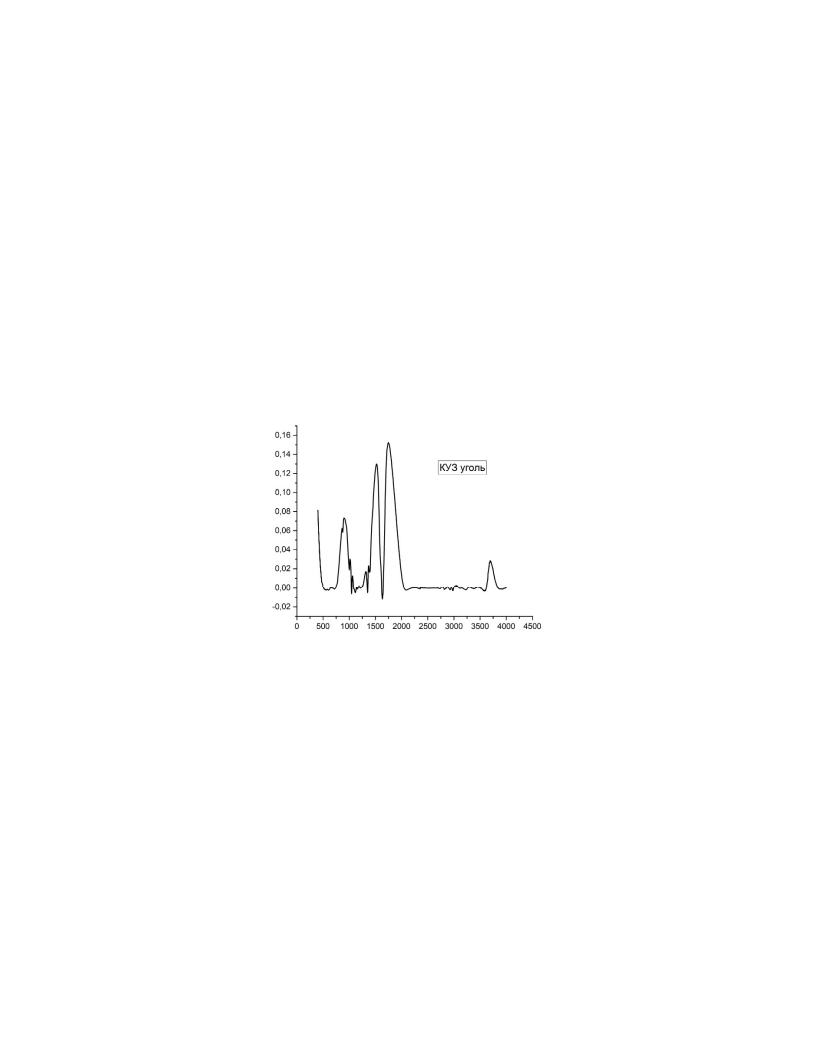
\includegraphics[width=0.5\textwidth]{media/gorn3/image12}
	\caption*{Рис. 4 - ИК спектры образцов углей}
\end{figure}

\begin{multicols}{2}
Как видно из рисунка 4, полоса в области 3800--3600 см⁻¹ свидетельствуют
о воде, связанная с поверхностью угля, или гидроксильными группами,
образованные при химических реакциях. В диапазоне 2000--1600 см⁻¹
наблюдаются поглощения, связанные с колебаниями C=O связей. Это могут
быть карбонильные соединения, такие как кетоны, альдегиды или
карбоксильные группы. В углях такие полосы могут возникать из-за наличия
кислородсодержащих функциональных групп, которые участвуют в процессах
окисления. Полоса в области 1600--1300 см⁻¹ отвечает за деформационные
колебания C--H и C=C связей в ароматических кольцах. Угли содержат
большое количество ароматических структур, и этот диапазон может
указывать на степень ароматичности углеродного скелета угля. Чем
интенсивнее полосы в этом диапазоне, тем выше содержание ароматических
углеродов. Диапазон 1000--750 см⁻¹ может указывать на наличие замещенных
бензольных колец (ароматических углеводородов) и колебания C--H в
плоскости кольца. Также здесь могут проявляться колебания
углеродно-кислородных связей в таких структурах, как эфиры или спирты,
если они присутствуют в угле.

{\bfseries Дифференциальная сканирующая калориметрия (ТГА)/ДСК анализ.}
ТГ/ДСК анализ проводился на приборе
LABSYS\textsuperscript{TM}EvoTG-DTA/DSC(SETARAM, Франция) для оценки
термической стабильности исследуемых образцов и изучения процесса их
разложения при нагреве. Образцы углей были помещены в тигли из оксида
алюминия и нагревались с постоянной скоростью 10°C/мин в атмосфере
воздуха до температуры 1000°C. В процессе измерялись изменения массы
образца, что позволило определить температуры, при которых происходят
основные стадии разложения органической материи, а также содержание
влаги, летучих веществ, фиксированного углерода и золы. ТГА также
позволил оценить стабильность органических компонентов угля и его
возможную реакционную способность. Полученные данные представлены в
рисунке 5.
\end{multicols}

\begin{figure}[H]
	\centering
	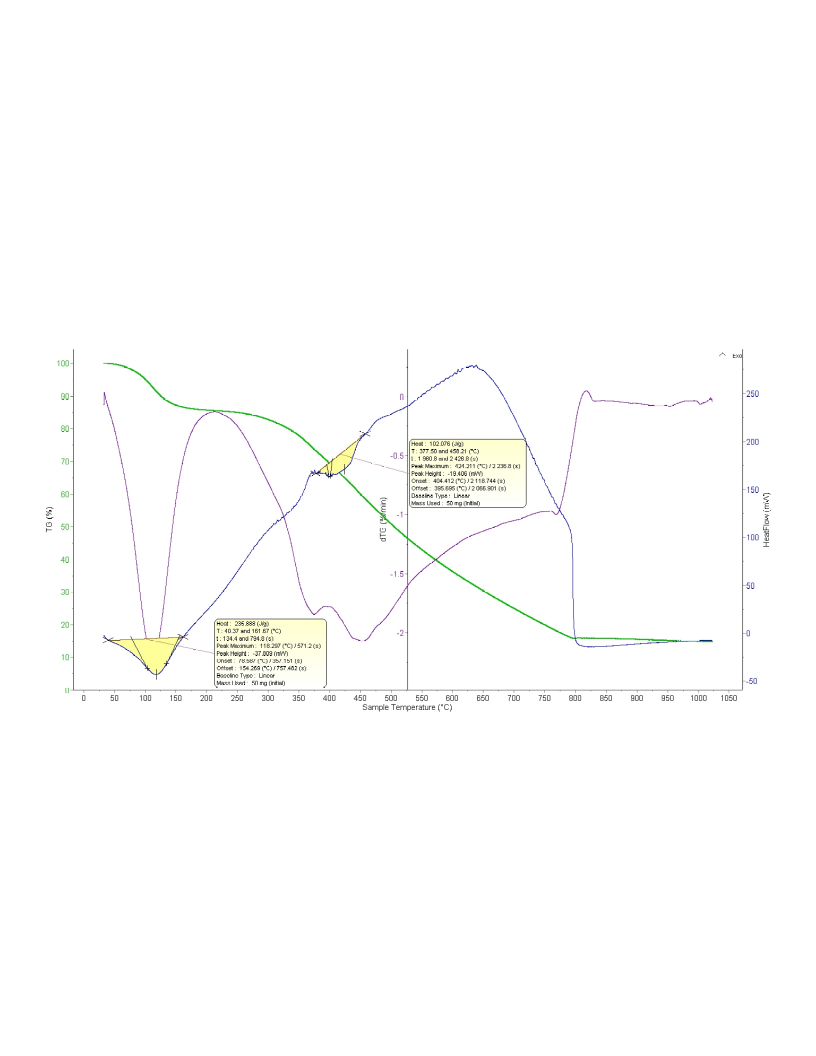
\includegraphics[width=0.8\textwidth]{media/gorn3/image13}
	\caption*{Рис. 5 - Результаты ТГ/ДСК анализа Кузнецкого угля}
\end{figure}

\begin{multicols}{2}
Из рисунка 5 можно заметить, что термическое разложение угля проходит в
несколько этапов, характеризующихся различными температурными
диапазонами и потерей массы. В диапазоне 32--213°C происходит удаление
влаги и легколетучих соединений. Потеря массы 14,5 \% связана с
испарением гигроскопической и связанной воды, а также возможным
удалением некоторых низкомолекулярных летучих соединений. На втором
этапе при 217--394°C с потерей массы 15\% происходит разложение
нестабильных углеводородов, выделение летучих веществ, включая
углеводороды, угарный газ (CO) и небольшое количество углекислого газа
(CO₂). Основная стадия пиролиза приходится на диапазон 400--820°C (54\%)
и характеризуется интенсивным разложением органической части угля с
образованием коксового остатка, значительного количества газообразных
продуктов и жидких конденсатов. В этот период разрушаются ароматические
структуры, выделяются газы, такие как CH₄, H₂, CO, CO₂, а также смолы и
полициклические углеводороды. После 820°C разложение угля, как правило,
завершается, и остаётся в основном минеральный остаток массой около
15\%.

Эндотермические пики на кривой дифференциальной сканирующей калориметрии
(ДСК) указывают на тепловые эффекты, сопровождающие разложение угля. Пик
при 40 --162°C связан с испарением влаги (гигроскопической и
капиллярно-связанной воды), а также, возможно, с удалением
низкомолекулярных летучих соединений. Высокая энтальпия процесса (235
Дж/г) указывает на значительные энергозатраты на испарение.
Эндотермический пик с поглощением теплоты 102 Дж/г в диапазоне
377--458°C может быть обусловлен разложением кислородсодержащих
функциональных групп органической массы угля. Также в этом диапазоне
происходит частичный пиролиз и выделение летучих веществ. Оба пика
подтверждают этапность термического разложения угля, соответствующую
данным термогравиметрического анализа (ТГА).

{\bfseries Вычисление количественного выхода гуминовых веществ из угольных
отходов.} В результате проведенных экспериментов из образцов углей
Кузнецкого месторождений были извлечены гуминовые кислоты методом
щелочного гидролиза. Из углей Кузнецкого месторождения массой 10 г было
получено 0,7 г гуминовых кислот (выход 7\%) (рис.6).
\end{multicols}

{\bfseries Рис.6 - Подкисление и осаждение гуминовых кислот}

\begin{multicols}{2}
В рамках оптимизации технологии экстракции гуминовых кислот
исследовались различные параметры процесса: концентрация щелочного
раствора (1--4\%), температура (20-80°C) и продолжительность реакции
(30--120 минут). Экспериментально было установлено, что наиболее полное
разделение гуматов натрия происходит при использовании 4\%-ного раствора
щелочи при температуре 80°C и времени реакции 120 минут.

Высокая концентрация щелочи способствует более полному извлечению
гуминовых кислот, однако повышение температуры обработки выше 80°C
приводит к снижению выхода гуматов натрия (с 4\% до 2\%) и значительному
изменению состава продуктов. Это связано с гидролизом и выщелачиванием
карбоксильных и полисахаридных фрагментов, что увеличивает относительное
содержание ароматических структур (до 44--45\%). Продление времени
реакции более 2 часов не оказывает значительного влияния на степень
извлечения гуминовых кислот.

{\bfseries Спектроскопическая оценка содержания гуминовых веществ и
исследование структурных характеристик.} В результате проведенных
экспериментов из образцов углей Кузнецкого месторождений были извлечены
гуминовые кислоты методом щелочного гидролиза. Полученные образцы
гуминовых кислот проанализированы методами ИК и ТГ/ДСК анализа (рис. 7,
8).
\end{multicols}

\begin{figure}[H]
	\centering
	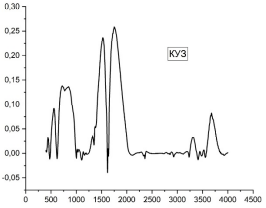
\includegraphics[width=0.8\textwidth]{media/gorn3/image18}
	\caption*{Рис. 7 - ИК спектры полученных гуминовых кислот}
\end{figure}

\begin{multicols}{2}
На рисунке 7 видно, что в диапазоне 3800--3550 см⁻¹ присутствует полоса
поглощения, связанные с колебаниями O--H групп. Эти полосы характерны
для гидроксильных групп (как в свободной воде, так и в водородных
связях), которые присутствуют в структуре гуминовых кислот. При
2100--1600 см⁻¹ наблюдаются полосы поглощения, принадлежащие к
карбоксильным кислотам, альдегидам, кетонам и сложным эфирам. Диапазон
1600-1250см⁻¹ отвечает за колебания ароматических C=C связей, что
характерно для гуминовых кислот, которые имеют в своей структуре
ароматические кольца. Также здесь могут проявляться деформационные
колебания C--O связей в карбоксильных и фенольных группах, что указывает
на наличие сложных кислородсодержащих функциональных групп в гуминовых
кислотах. При 1000-600см⁻¹ можно наблюдать полосы поглощения, связанные
с деформационными колебаниями C--H в ароматических кольцах, а также
колебания C--O--C связей в сложных эфирах и эфирных группах.
Низкочастотный диапазон 600-500-см⁻¹ связан с колебаниями вне плоскости
C--H в ароматических системах, а также колебаниями, связанными с
деформациями C--C связей в углеродных цепях. Термогравиметрический
анализ гуминовых кислот проводился в инертной среде до температуры
1000°С.

Определение функциональных групп угля важно для понимания его
реакционной способности, способности к сорбции, горению, коксованию и
другим технологическим процессам. Исследование состава функциональных
групп угля Кузнецкого месторождения позволяет оценить его потенциал как
топлива и сырья для химической промышленности, а также выбрать
оптимальные методы его переработки.

Методы, описанные выше, обеспечивают комплексный подход к исследованию
угля и помогают лучше понять его химическую природу и потенциал
использования в различных отраслях. Полученные данные представлены в
рисунке 8.
\end{multicols}

\begin{figure}[H]
	\centering
	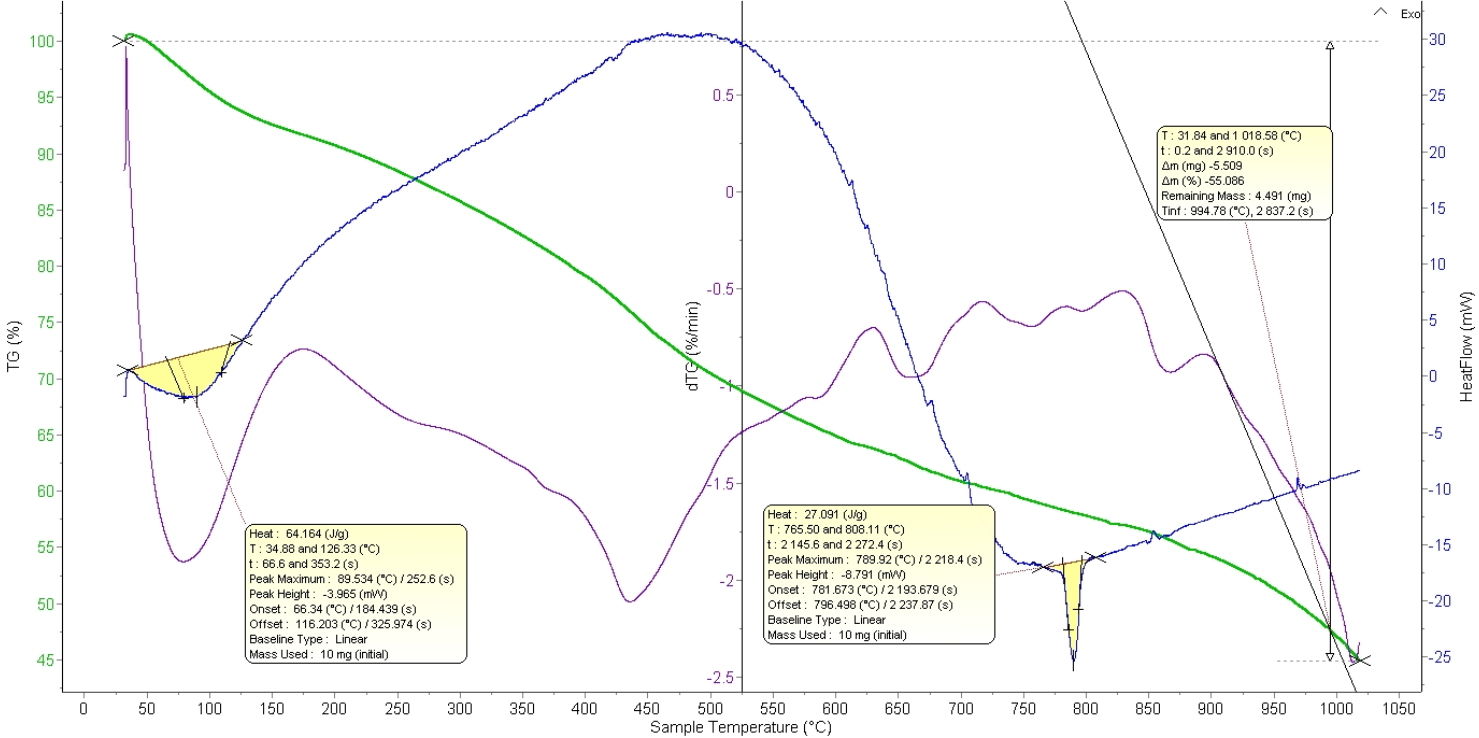
\includegraphics[width=0.8\textwidth]{media/gorn3/image19}
	\caption*{Рис. 8 - Результаты ТГ/ДСК анализа образцов гуминовых кислот (KUZ)}
\end{figure}

\begin{multicols}{2}
Как видно из кривых термогравиметрического анализа гуминовых кислот в
диапазоне 30 \textasciitilde{} 175°С наблюдается незначительное
изменение массы 7\% вероятно связанное с остатками воды. Далее
разложение образца происходит в две стадии. Первая стадия при 175-525°С
с потерей массы 23\% сопровождается разложением легколетучих веществ и
функциональных групп, таких как карбоксильные, фенольные и метоксильные
группы. Также разрушаются небольшие органические молекулы, связанные с
ароматическими структурами, что приводит к существенной потере массы.
Эта стадия характеризуется выделением воды, углекислого газа и других
низкомолекулярных газов. Далее при температурах 550-1000°C происходит
разрушение более стабильных ароматических структур и конденсированных
полициклических систем. Что приводит к дальнейшей потере массы и
образованию углеродных остатков (45\% от общей массы). Основные процессы
включают углерификацию (превращение органического вещества в углерод) и
образование устойчивого остатка, напоминающего кокс. Эти стадии отражают
последовательное термическое разложение гуминовых кислот, начиная от
легких функциональных групп до стабильных углеродных структур.

На кривой ДСК гуминовых кислот наблюдается тепловой эффект при 35--126°C
который связан с удалением влаги. Энтальпия 64 Дж/г указывает на
относительно небольшие затраты тепла, характерные для процессов
дегидратации. При 765--808°C присутствует небольшой эндотермический пик,
который возможно связан с разложением остаточных устойчивых структур,
например, ароматических фрагментов с высокой степенью конденсации.
Низкая энтальпия (27 Дж/г) указывает на небольшие энергозатраты, что
характерно для завершающих стадий разложения. Таким образом данные
показывают, что термическое разложение гуминовых кислот происходит
поэтапно, сначала с потерей влаги, затем с разрушением функциональных
групп, аналогично процессам в углях, но с более низкими энергозатратами
из-за меньшей степени ароматизации структуры.

{\bfseries Определение химического состава гуминового продукта}. Далее с
помощью элементного анализатора CHNS-O UNICUBE (Elementar
Analysensysteme GmbH) были определены содержания углерода (C), водорода
(H), азота (N), серы (S) и кислорода (O) в гуминовых кислотах (ГК),
полученных из бурых углей месторождений Кузнецкого. Исследование
проводилось для определения элементного состава этих кислот, что
позволяет оценить их химические свойства и потенциальные области
применения в сельском хозяйстве.

В таблице 3 приведены средние значения содержания химических элементов в
процентах для гуминовых кислот, полученных с Кузнецкого месторождений.
\end{multicols}

{\bfseries Таблица 3 -- Средние значения содержания кислорода (O), углерода (C), водорода (H), азота (N) и серы (S) в гуминовых кислотах}


\begin{multicols}{2}
В гуминовой кислоте из Кузнецкого месторождения содержание углерода
составляет 49.605\%. Это может указывать на более высокую степень
ароматичности или полимеризации органического материала в Кузнецких
углях. В гуминовой кислоте из Кузнецкого месторождения содержание
углерода составляет 49.605\%. Это может указывать на более высокую
степень ароматичности или полимеризации органического материала в
Кузнецких углях. Содержание водорода в кислотах, полученных из
Кузнецкого месторождения, составляет 3,071\%. Концентрация азота в
гуминовой кислоте данного месторождения равна 0,93\%. Повышенное
содержание азота может свидетельствовать о наличии значительного
количества аминогрупп или белковых соединений в образце. В анализируемом
образце содержание серы составляет 0,391\%, что, вероятно, обусловлено
присутствием сульфидных или органических серосодержащих соединений.
Гуминовая кислота из Кузнецкого месторождения характеризуется повышенным
содержанием кислорода (45,263\%), что может свидетельствовать о наличии
карбоксильных групп, способствующих увеличению кислотности и реакционной
способности вещества.

Таким образом, гуминовая кислота из Кузнецкого месторождения, благодаря
высокому содержанию углерода, низкому содержанию азота и серы, имеет
более сбалансированный элементный состав, что делает её перспективной
для использования в качестве компонента органоминеральных мелиорантов.
Она способна эффективно улучшать физико-химические свойства почвы и
обеспечивать растения необходимыми элементами питания.

{\bfseries Выводы.} В ходе исследования гуминовых кислот, выделенных из
бурого угля Кузнецкого месторождения, были получены данные о их составе,
структуре и функциональных свойствах. Применение методов элементного
анализа, инфракрасной (ИК) спектроскопии, термогравиметрического анализа
(ТГА) и дифференциальной сканирующей калориметрии (ДСК) позволило
охарактеризовать химический состав гуминовых кислот и определить наличие
карбоксильных и фенольных групп.

Результаты исследования показали, что выход гуминовых кислот из бурого
угля Кузнецкого месторождения составляет 7\%, что является сравнительно
низким показателем. Несмотря на наличие функциональных групп,
определяющих кислотность и способность к сорбции тяжелых металлов, такой
низкий выход ограничивает их практическое применение в качестве
самостоятельного источника гуминовых веществ. Таким образом, бурый уголь
Кузнецкого месторождения нельзя рассматривать как перспективное сырье
для промышленного получения гуминовых кислот. В дальнейшем целесообразно
исследовать альтернативные методы увеличения выхода гуминовых веществ
либо изучить возможность использования других углеродных материалов с
более высокой эффективностью экстракции гуминовых соединений.

\emph{{\bfseries Финансирование.} Данное исследование выполнено в рамках
программы целевого финансирования по проекту ИРН BR24992961 «Разработка
новых технологий переработки угольных отходов с использованием биосистем
в органоминеральные удобрения для повышения плодородия почвы и
урожайности сельскохозяйственных культур».}
\end{multicols}

\begin{center}
{\bfseries References}
\end{center}

\begin{references}
1. Tyanakh S., Baikenov M.I., Ma Feng Yun, Khamitova T. O., Balpanova
N.Zh., Tulebayeva B., \\Kyzkenova A., Karimova A.B., Rakhimzhanova N.Zh.,
Kochegina E.V\emph{.} Kinetic of oil sludge thermolysis process in
presence of nickel, cobalt and iron-supported microsilicate // Polish
Journal of Chemical \\Technology.- 2023.- Vol.23(3).- P.101-109. DOI
\href{https://doi.org/10.2478/pjct-2023-0030}{10.2478/pjct-2023-0030}

2. Baikenov M.I., S. Tyanakh, Ma Feng-Yun, Gulmaliev A.M., Makasheva
A.M., Khamitova T.O. \& Malyshev V.P. Viscosity model for the middle
fraction of Atasu-Alashankou oil sludge // Mendeleev Communications.-
2024.-Vol. 34(3).P.446 - 449.
\href{https://doi.org/10.1016/j.mencom.2024.04.043}{DOI
10.1016/j.mencom.2024.04.043}

3. Tyanakh S., Baikenov M.I., Gulmaliev A.M., Ma, Feng-Yun, Musina G.,
Khamitova T.O., \& Bolatbay A.N\emph{.} Kinetics of Thermolysis of a
Low-Temperature Tar in the Presence of a Catalyzer Agent with Deposited
Metals // Bulletin of the University of Karaganda Chemistry.-2022.-№
4(108). - P. 89-98. \href{https://doi.org/10.31489/2022Ch4/4-22-19}{DOI
10.31489/2022Ch4/4-22-19}

4. Margaret Suárez Muñoz, Clara Melián Rodríguez, Alina Gelen Rudnikas
and other autors. \\Physicochemical characterization, elemental speciation
and hydrogeochemical modeling of river and peloid sediments used for
therapeutic uses // Applied Clay Science. - 2015.- Vol. 104.- P. 36-47.
DOI \\10.1016/j.clay.2014.11.029

5. Chen Y., Banin A., Schnitzer M. Use of the scanning electron
microscope for structural studies on soil and soil components //
Scanning electron microscopy. Рart 3: Proceeding of the workshop on
techniques for particulate matter studies on SEM.-1976.- Р.425 - 432.

6. Kairbekov Zh.K. Pererabotka tverdyh gorjuchih iskopaemyh // Kniga, --
Almaty: tipografija «BTS print».- 2014. -S. 260.{[}in Russian{]}

7.
\href{https://www.scopus.com/authid/detail.uri?authorId=55910705200}{Kairbekov
Zh.K.},
\href{https://www.scopus.com/authid/detail.uri?authorId=57201691853}{Suimbaeva
S.M.},
\href{https://www.scopus.com/authid/detail.uri?authorId=56600659100}{Dzheldybaeva
I.M.},
\href{https://www.scopus.com/authid/detail.uri?authorId=56600640700}{Kairbekov
A.Zh.},
\href{https://www.scopus.com/authid/detail.uri?authorId=58021595400}{Abil' Mazhinova
D.Z.} \\Antioxidant Activity and Bioavailability of Humic Substances of
Low-Mineralized Sulphide Mud // \\Engineered Science.- 2023.- № 25.- P.
941-948. DOI \href{http://dx.doi.org/10.30919/es941}{10.30919/es941}

8.
\href{https://www.scopus.com/authid/detail.uri?authorId=56600659100}{Dzheldybaeva
I.M.},
\href{https://www.scopus.com/authid/detail.uri?authorId=55910705200}{Kairbekov
Z.K.},
\href{https://www.scopus.com/authid/detail.uri?authorId=7003481604}{Maloletnev
A.S.},
\href{https://www.scopus.com/authid/detail.uri?authorId=58021595400}{Abil'mazhinova
D.Z.},
\href{https://www.scopus.com/authid/detail.uri?authorId=57201691853}{Suimbaeva
S.M.} \\Physicochemical and Antioxidant Properties of Humic Substances
from Coals of the Oy-Karagay and Kiyakty Deposits in the Republic of
Kazakhstan // Solid Fuel Chemistry.- 2022.-Vol. 56.- P. 471-477.
\href{https://doi.org/10.3103/S0361521921060033}{DOI
10.3103/S0361521921060033}

9. Kairbekov Zh.K., Toktamysov M.T., Zhalgasuly N., Eshova
Zh.T.~Kompleksnaya pererabotka burykh uglei Tsentral'nogo
Kazakhstana~(Integrated Processing of Brown Coal from Central
Kazakhstan) // Almaty: Izd. KazNU. -- 2014.

10. Arziev Zh.A. Ugli Kyrgyzstana kak osnova dlja poluchenija guminovyh
udobreniĭ i stimuljatorov rosta rasteniĭ // Sovremennye problemy nauki i
tehniki: Sb. nauchn. tr. regional' noĭ nauchn. - teoret.
konf. / Zhalalabatskiĭ gos.tehn.in-t.- Zhalalabat.- 2002.- № 1.- S.34 -
38.{[}in Russian{]}
\end{references}

\begin{authorinfo}
\emph{{\bfseries Сведения об авторах}}

Науанова А.П.-доктор биологических наук, профессор, Казахский
агротехнический исследовательский университет им. Сейфуллина, Астана,
Казахстан, е-mail:
\href{mailto:nauanova@mail.ru}{\nolinkurl{nauanova@mail.ru}};

Хамитова Т.О.- PhD, и.о. ассоцированного профессора, Казахский
агротехнический исследовательский университет им. Сейфуллина, Астана,
Казахстан, е-mail:
\href{mailto:khamitova.t@inbox.ru}{\nolinkurl{khamitova.t@inbox.ru}};

Парманбек Н.- PhD, инженер, Институт ядерной физики, Алматы, Казахстан,
е-mail:
\href{mailto:parmanbek.nursanat@gmail.com}{\nolinkurl{parmanbek.nursanat@gmail.com}};

Тянах С.-Магистр, докторант, Карагандинский университет имени
Е.А.Букетова, Караганда, Казахстан, е-mail:\\
\href{mailto:saika_8989@mail.ru}{\nolinkurl{saika\_8989@mail.ru}};

Касенов Р.З.- доцент, Карагандинский университет имени Е.А.Букетова,
Караганда, Казахстан, е-mail:\\
\href{mailto:r_z_kasenov@mail.ru}{\nolinkurl{r\_z\_kasenov@mail.ru}};

Давренбеков С.Ж.- ассоцированный профессор, Карагандинский университет
имени Е.А.Букетова, Караганда, Казахстан, е-mail:
\href{mailto:sdavrenbekov@mail.ru}{\nolinkurl{sdavrenbekov@mail.ru}};

Болатбай А.Н.-магистр, докторант, Карагандинский университет имени Е.А.
Букетова, Караганда, Казахстан, е-mail:
\href{mailto:abylai_bolatabai@mail.ru}{\nolinkurl{abylai\_bolatabai@mail.ru}};

Тулеуов У. Б.-научный сотрудник, НИИ химических проблем, Караганда,
Казахстан, е-mail:
\href{mailto:bekalols1@gmail.com}{\nolinkurl{bekalols1@gmail.com}}

\emph{{\bfseries Information about the authors}}

Nauanova A. P. - doctor of Biological Sciences, Professor, NCJSC
«S.Seifullin Kazakh Agro Technical Research University», Astana,
Kazakhstan, e-mail:
\href{mailto:nauanova@mail.ru}{\nolinkurl{nauanova@mail.ru}};

Khamitova T.O.-PhD, acting associate professor, NCJSC «S.Seifullin
Kazakh Agro Technical Research University», Astana, Kazakhstan, e-mail:
\href{mailto:khamitova.t@inbox.ru}{\nolinkurl{khamitova.t@inbox.ru}};

Parmanbek N.-PhD, engineer, The Institute of Nuclear Physics, Almaty,
Kazakhstan, e-mail:
\href{mailto:parmanbek.nursanat@gmail.com}{\nolinkurl{parmanbek.nursanat@gmail.com}};

Tyanakh S.- master, doctoral student, E.A. Buketov Karagandy University,
Karaganda, Kazakhstan, e-mail:
\href{mailto:saika_8989@mail.ru}{\nolinkurl{saika\_8989@mail.ru}};

Kasenov R.Z.- docent, E.A. Buketov Karagandy University, Karaganda,
Kazakhstan, e-mail:
\href{mailto:r_z_kasenov@mail.ru}{\nolinkurl{r\_z\_kasenov@mail.ru}};

Daurenbekov S.Z.-Associate Professor, E.A. Buketov Karagandy University,
Karaganda, Kazakhstan, e-mail:\\
\href{mailto:sdavrenbekov@mail.ru}{\nolinkurl{sdavrenbekov@mail.ru}};

Bolatbay A.N.-master, doctoral student, E.A. Buketov Karagandy
University, Karaganda, Kazakhstan, e-mail:\\
\href{mailto:abylai_bolatabai@mail.ru}{\nolinkurl{abylai\_bolatabai@mail.ru}};

Tuleuov U. B.- researcher, Research Institute of Chemical Problems,
Karaganda, Kazakhstan, e-mail:
\href{mailto:bekalols1@gmail.com}{\nolinkurl{bekalols1@gmail.com}}
\end{authorinfo}
